\subsection{Motivation \& Background}

When simulating problems in computational fluid dynamics involving complex
geometries, numerical difficulties are often encountered that require
employing one of a number of different approaches to mitigate loss of accuracy
due to poor spatial resolution. While finite-difference approaches to spatial
discretization are popular due to their simplicity and efficiency when working
with smooth solutions, their geometric flexibility is typically limited in spite
of the well-documented ability to use coordinate transforms to create intricate
curvilinear meshes, as well as the ability to use overset meshes to produce
higher resolution in a particularly troublesome section of the spatial domain.

In particular, the SBP-SAT methodology pioneered by, which mimics
integration-by-parts in the discrete sense and features weak enforcement of
boundary conditions to produce provable stability via the energy method,
is an attractive one when it comes to finite differences, and its geometric
flexibility has recently been further improved by a large body of work in creating
accurate and stable interfaces between nonconforming blocks. In 2010, Mattsson and
Carpenter introduced interpolation operators that maintained the stability and
high-order accuracy of the underlying spatial scheme on each block, but the
resulting scheme is based on a fixed refinement ratio and the requirement that
the blocks conform at their corners (the latter of these characteristics was
later removed by Nissen et. al in 2014).

Meanwhile, another attractive approach to modeling complex geometries more efficiently
with a localized spatial discretization change is to create a hybrid spatial
discretization that requires an interface between a high-order finite difference
method (used away from the complex boundary) and an unstructured mesh with
improved geometric flexibility (used near the complex boundary). Nordstrom and Gong
proposed such a scheme in 2006, coupling a high-order finite difference method
and a second-order finite volume scheme. More recently, in 2016, Kozdon and Wilcox
developed an interface method between SBP finite-difference blocks that was based
on projection into an intermediate "glue" grid characterized by piecewise polynomials,
with the method also extending to the coupling between SBP finite-difference methods
and discontinuous Galerkin methods. In this work, the interface method was proven
to be stable via the energy method, but the projection operators were not fully
determined and were based in part on an optimization procedure focused on driving
the product of the projection matrices closer to an identity operation. Furthermore,
the method was not extended to three dimensions, and the method is reduced to
first order accuracy if the continuous coordinate transforms on either side
of the interface are dissimilar.

\begin{figure}
\centering
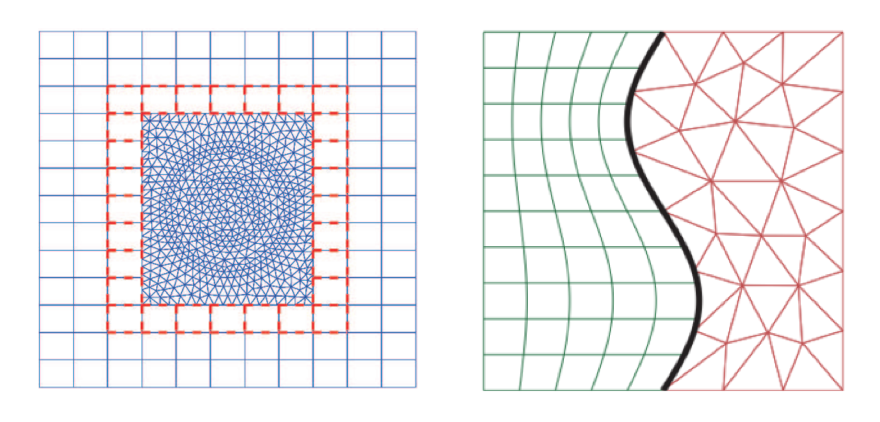
\includegraphics[width=0.8\linewidth,trim=4 4 4 4,clip]{figures/nonconforming_samples.png}
\caption{Two examples demonstrating use of nonconforming interfaces. Left: Zhu, Chen, Zhong, and Liu \cite{zhu2011hybrid}.
	 Right: Kozdon and Wilcox \cite{kozdon2016stable}}
\label{fig:nonconforming_samples}
\end{figure}

Since, Friedrich et. al extended the method(s) of Kozdon and Wilcox to make the
projection process degree-preserving (a characteristic that had been
previously shown to be problematic by Lundquist and Nordstrom) as well as
energy-stable and conservative, but their approach still results in projection
operators that are not fully determined, relying upon an optimization procedure
to produce the operators that give their results. Furthermore, unlike Kozdon
and Wilcox, they fail to extend their method to hybrid structured-unstructured
discretizations.

\subsubsection{Goals, Bounds, and Impact}

This section of the proposal targets a lack of fully determined high-order
accurate and provably stable interface conditions between structured and unstructured
meshes for computational fluid dynamic simulations. In particular, our aim
is to create a provably stable, accurate, and fully determined interface between
summation-by-parts finite difference discretizations (structured) and discontinuous
Galerkin methods (unstructured) that doesn't rely on optimization to establish its
projection operators. Achieving this would provide a more robust option to create
localized areas of unstructured meshing (with superior flexibility for discretizing
complex boundaries/geometries) in existing simulations, providing an alternative to
comparatively less flexible overset curvilinear meshes or multiblock conforming/nonconforming
finite difference schemes.

%===========================================================================
\subsection{Governing Equations}

The initial problem for which our new hybrid method will be targeted is
the acoustic wave equation in two dimensions, in first-order form:
\begin{align}
&\rho \frac{\partial v_{i}}{\partial t} + \frac{\partial p}{\partial x_{i}} = 0 \hspace{2mm} (i = 1, 2), \\
&\frac{\partial p}{\partial t} + \lambda \left(\frac{\partial v_{1}}{\partial x_{1}} + \frac{\partial v_{2}}{\partial x_{2}} \right) = 0
\end{align}

As in \cite{kozdon2016stable}, our aim will be to prove the semi-discrete hybrid discretization
stable via the energy method by proving that
\begin{align}
\frac{d\mcl{E}}{dt} \leq 0
\end{align}
where the total energy of the semi-discrete system $\mcl{E}$ is obtained by summing the
energy $E$ of each discretization block:
\begin{align}
\mcl{E} = \sum_{blocks} E
\end{align}

%===========================================================================
\subsection{Numerical Methods}

\subsubsection{Summation-by-Parts Operators}

For the structured discretization that makes up one component of the proposed hybrid, we make use of several
finite difference operators that possess the summation-by-parts (SBP) property. Taking two matrices
${P,Q}$, we here state that these two matrices are SBP matrices of order $p$ provided 
\begin{itemize}
\item $P^{-1}Q v$ is an order $h^{p}$ approximation to $\partial/\partial x$, where $h$ is the spatial step size in one dimension.
\item P is a symmetric positive-definite matrix.
\item $Q + Q^{T} = \text{diag}(-1,0,0,...,0,1)$.
\end{itemize}
These conditions together ensure that the discrete version of the integration by parts property holds; that is,
\[\langle P^{-1}Q x , y\rangle_{P} = x_{N} y_{N} -  x_{1} y_{1} - \langle x,P^{-1}Q y\rangle _{P}. \]

The resulting operators can be either explicit (in this case, $P$ is purely diagonal) or implicit.
This theory, originally presented in \cite{strand1994summation}, can also be extended to higher
dimensions using Kronecker products.  For example, in two dimensions, the matrices $H^{-1} G_x$
and $H^{-1} G_y$ define the $x$- and $y$- derivatives on a two-dimensional grid:
\begin{align}
H = P_{x} \otimes P_{y} \notag \\
G_{x} = Q_{x} \otimes P_{y} \notag \\
G_{y} = P_{x} \otimes Q_{y} \notag
\end{align}
Note that this formulation assumes that we have ${P_{x},Q_{x}}$, a pair of $n_{x} \times n_{x}$ SBP
matrices of approximation order $p$, and ${P_{y},Q_{y}}$, a pair of $n_{y} \times n_{y}$ SBP matrices
of approximation order $q$. Finally, we also note that these SBP operators do not guarantee strict
stability for an initial boundary value problem. We must also apply the boundary conditions using a
formulation that permits an energy estimate. More information on these boundary conditions, called
simultaneous approximation term (SAT) boundary conditions, can be found at \cite{svard2007stable},
\cite{svard2008stable}, and \cite{bodony2010accuracy}.

More information on SBP operators of various order, including the coefficients themselves, can be found
in \cite{strand1994summation}, \cite{carpenter1993time}, \cite{mattsson2004stable}. For this work,
we will employ diagonal-norm SBP operators for the finite difference discretizations.

The SBP-SAT spatial discretization of the governing equations in the previous section,
in two dimensions and including the effect of coordinate transform from the physical
space to a reference space, is given by
\begin{align}
  &\rho J \frac{d v_{i}}{dt}
	+ D_{1} J \frac{ \partial \xi_{1}}{\partial x_{i}} p
  + D_{2} J\frac{\partial \xi_{2}}{\partial x_{i}} p =
  - {H}^{-1}\mcl{F}_{v_{i}}, \quad i=1,2,\\
  &J\frac{\partial p}{\partial t} +\lambda\left(
    J\frac{\partial \xi_{1}}{\partial x_{1}} D_{1} v_{1}
  + J\frac{\partial \xi_{2}}{\partial x_{1}} D_{2} v_{1}
  + J\frac{\partial \xi_{1}}{\partial x_{2}} D_{1} v_{2}
  + J\frac{\partial \xi_{2}}{\partial x_{2}} D_{2} v_{2}
  \right)
  =
  -\lambda H^{-1} \mcl{F}_{p}.
\end{align}
Here, we have defined the matrices
\begin{align}
  H     =\;& H_{N_{1}}\otimes H_{N_{2}},&
  D_{1} =\;& D_{N_{1}}\otimes I_{N_{2}},&
  D_{2} =\;& I_{N_{1}}\otimes D_{N_{2}},&
\end{align}
The penalty terms in the above equations implement the boundary conditions via the
SAT method, and are defined as follows:
\begin{align}
  \mcl{F}_{v_{i}} =\;&
    \left(  e_{W} \otimes \mcl{F}^{W}_{v_{i}} \right)
  + \left(  e_{E} \otimes \mcl{F}^{E}_{v_{i}} \right)
  + \left( \mcl{F}^{S}_{v_{i}} \otimes e_{S} \right)
  + \left( \mcl{F}^{N}_{v_{i}} \otimes e_{N} \right),\\
  \mcl{F}_{p} =\;&
    \left( e_{W} \otimes \mcl{F}^{W}_{p} \right)
  + \left( e_{E} \otimes \mcl{F}^{E}_{p} \right)
  + \left( \mcl{F}^{S}_{p} \otimes e_{S} \right)
  + \left( \mcl{F}^{N}_{p} \otimes e_{N} \right).
\end{align}

\subsubsection{Discontinuous Galerkin Method}

The discontinuous Galerkin method we will target our interface method(s) to
will be briefly summarized here. As in Kozdon and Wilcox, we denote a DG
element $\Omega_e$ with triangular reference element $\tilde{\Omega}$.
\begin{align}
&\int_{\tilde{\Omega}} \left[ w_{i}\rho J \frac{\partial v_{i}}{\partial t}
- \frac{\partial w_{i}}{\partial \xi_{1}}J\frac{\partial \xi_{1}}{\partial x_{i}} p
- \frac{\partial w_{i}}{\partial \xi_{2}}J\frac{\partial \xi_{2}}{\partial x_{i}} p\right]\;dA
=
-\int_{\partial \tilde{\Omega}} w_{i} S_{J} n_{i} p^*ds.
\end{align}
On each element, we therefore have
\begin{align}
  \rho M_{J} \frac{d v_{i}}{dt} =&
  D_{1}^{T} M_{1i} p
  + D_{2}^{T} M_{2i} p
  - \sum_{K=1}^{3} L_{K}^{T} P_{bc}^{T} n_{iK}
  \Omega_{bc} S_{JK} p_{K}^{*},\\
  \notag
  M_{J} \frac{dp}{dt} =&
  -\lambda\left(
    M_{11} D_{1} v_{1}
    +
    M_{21} D_{2} v_{1}
    +
    M_{12} D_{1} v_{2}
    +
    M_{22} D_{2} v_{2}
  \right)\\
  &- \sum_{K=1}^{3}\lambda L_{K}^{T} P_{bc}^{T} \Omega_{bc}
  S_{JK} \left(v_{K}^* - v_{K}^{-}\right),
\end{align}
where the vector $v_{K}^{-}$ is the normal component of velocity along
edge $K$ of the element evaluated at the cubature points:
\begin{align}
  v^{-}_{K} = n_{1K} P_{bc} L_{K} v_{1}
    + n_{2K} P_{bc} L_{K} v_{2}.
\end{align}
Here $L_{K}$ takes the volume terms to edge $K$ of the element
and $L_{K}^{T}$ takes edge $K$ terms to the volume; this is similar
to the behavior of $e_{W/E} \otimes I$ and  $I \otimes
e_{N/S}$ in the SBP method.
Also as in the SBP method, $D_{1}$ and $D_{2}$ are the reference
element differentiation matrices for the two reference coordinate directions.
Since we will be using curved triangular elements, integration is done using
a cubature in the volume and quadratures along the edges of the elements.
Thus we introduce the projection matrices
$P_{c}$ and $P_{bc}$ that project from the volume and edge
approximations to the volume and edge cubature points, respectively. At the
cubature locations, the matrices $\Omega_{c}$ and $\Omega_{bc}$ are
diagonal matrices of the integration weights for the volume and an edge,
respectively.  To ensure stability of the method, we will assume that
$\Omega_{c}$ and $\Omega_{bc}$ are positive definite. The
element mass matrices in the discretization are defined as
\begin{alignat}{2}
  M_{J}  &= P_{c}^{T} \Omega_{c} J P_{c},\quad&
  M_{ij} &= P_{c}^{T} \Omega_{c} J
                  \frac{\partial \xi_{i}}{\partial x_{j}} P_{c}.
\end{alignat}
Here the diagonal matrices $J$ and $\frac{\partial \xi_{i}}{\partial x_{j}}$ are,
respectively, the Jacobian determinant and metric derivatives defined at the
cubature points. The diagonal matrices $S_{JK}$ and $n_{iK}$
are the surface Jacobian and the components of the unit normal for edge $K$,
respectively, defined at the cubature points.

Defining the energy in a DG element as
\begin{align}
  E =
  \frac{\rho}{2}v_{1}^{T}M_{J}v_{1}
  + \frac{\rho}{2}v_{2}^{T}M_{J}v_{2}
  + \frac{1}{2\lambda}p^{T}M_{J}p
\end{align}
as well as the edge projected pressures
\begin{align}
  p_{K}^{-} = P_{bc}L_{K} p,
\end{align}
then the single DG block discretization has the energy dissipation rate
\begin{align}
  \frac{dE}{dt} = & \sum_{K=1}^{3} \mcl{D}_{K},\\
  \label{eqn:disp:edge:dg}
  \mcl{D}_{K} = &
  - {\left(v_{K}^{-}\right)}^{T}\Omega_{bc}S_{JK}p_{K}^{*}
  - {\left(p_{K}^{-}\right)}^{T}\Omega_{bc}S_{JK}
  \left(v^{*}_{K} - v^{-}_{K}\right).
\end{align}

\subsubsection{Interface Method}

The key contribution of this work will be construction of an interface
between the structured (finite difference SBP) and the unstructured (DG)
spatial discretizations that is stable and accurate. This interface will
be defined by operators $P_{a2b}$ and $P_{b2a}$ that project the solution
along the edge of discretization $a$ into discretization $b$, and vice versa.

A reasonable starting point for establishing such projection operators, then - 
or at least a reasonable starting point for establishing the conditions necessary
to create stable and accurate ones - is with the projection operators of Kozdon
and Wilcox \cite{kozdon2016stable}. As detailed in their paper, these operators
rely primarily upon the principle of projecting solutions from either discretization
first into an intermediate "glue" space of piecewise continuous polynomials
before projecting the solution onto the other nonconforming discretization. The
critical condition that allows proof of stability is referred to as the
\emph{compatibility condition}, and amounts to a simple relation between the
grid-to-glue and glue-to-grid projection operators, the mass matrix of the
piecewise polynomial description used in the glue layer, and a norm operator
$H$:
\begin{align}
P_{f2g}M = P_{g2f}^{T}H
\end{align}
In the case of SBP finite difference discretizations, the norm $H$ is equivalent
to the SBP-norm $P$, which for the purposes of this work we will take to be
a diagonal matrix. In the case of discontinuous Galerkin, this $H$ operator is
the diagonal matrix of integration weights at the cubature points at a single
DG element edge.

This compatibility condition, used in conjunction with the per-block semi-discrete
expressions for energy, is what allows for energy stability to be proven, and
as a result, this condition is used as an explicit constraint when constructing the
projection operators $P_{f2g}$ and $P_{g2f}$ themselves. The construction, which is
laid out in further detail in \cite{kozdon2016stable}, employs a Legendre polynomial
basis on the glue grid, and defines interior and boundary accuracy conditions when
projecting from grid to glue (and vice versa) that match those of corresponding SBP
diagonal-norm operators of the same order.

These conditions, in conjunction with symmetry conditions and a set of unknowns as
defined in the figure below, result in a \emph{non-square} system featuring more
unknowns than constraints, in particular near the boundary stencils. Given the
underdetermined nature of the system, the authors then use an optimization procedure
aimed at minimizing the distance between the nearest eigenvalues of $B =
P_{f2g}P_{g2f}$ to produce the final projection operators for a given order.

With all of this borne in mind, our primary goal for the interface method, then,
is to obtain projection operators that maintain the provable energy stability
of Kozdon and Wilcox, which are also
\begin{itemize}
\item{obtained from a construction procedure that is demonstrably \emph{unisolvent},
      with an equal number of constraints and unknowns resulting in a square system
      of equations}
\item{therefore not based on optimization}
\item{able to provide "round-trip" fidelity of projection, meaning that projection
      from the grid to the glue, and then back to the grid, results in a solution
      identical to the starting point.}
\end{itemize}
The strategy for pursuance of these goals begins with consideration of the
\emph{interior} projection operator only, given the simplicity of the existing
interior stencil relative to the boundary (which features many more unknowns).
Noting also that the compatibility condition disallows us from obtaining
exact "round-trip" projection, other conditions may be considered based
on the energy relation.

%===========================================================================
\subsection{Validation}

The test problem for validation will match that of \cite{kozdon2016stable},
modeling the two-dimensional acoustic wave equation in first-order form with
the following initial condition:
\begin{align}
  p(x_{1},x_{2},0) &=
  \cos\left(k_{1} x_{1}\right)\cos\left(k_{1} x_{2}\right)
  +
  \sin\left(k_{2} x_{1}\right)\sin\left(k_{2} x_{2}\right),\\
  v_{i}(x_{1},x_{2},0) &= 0,~ \quad i=1,2,
\end{align}
where $k_{1} = \pi/2$ and $k_{2} = \pi$. All exterior boundary conditions are
zero pressure (free-surface) conditions. The exact solution of this problem is
\begin{align}
  p(x_{1},x_{2},t) &=
  \cos\left(\omega_{1} t\right)
  \cos\left(k_{1} x_{1}\right)\cos\left(k_{1} x_{2}\right)
  +
  \cos\left(\omega_{2} t\right)
  \sin\left(k_{2} x_{1}\right)\sin\left(k_{2} x_{2}\right),\\
  v_{1}(x_{1},x_{2},t) &=
  \frac{k_{1}}{\omega_{1}} \sin\left(\omega_{1} t\right)
  \sin\left(k_{1} x_{1}\right)\cos\left(k_{1} x_{2}\right)
  -
  \frac{k_{2}}{\omega_{2}} \sin\left(\omega_{2} t\right)
  \cos\left(k_{2} x_{1}\right)\sin\left(k_{2} x_{2}\right),\\
  v_{2}(x_{1},x_{2},t) &=
  \frac{k_{1}}{\omega_{1}} \sin\left(\omega_{1} t\right)
  \cos\left(k_{1} x_{1}\right)\sin\left(k_{1} x_{2}\right)
  -
  \frac{k_{2}}{\omega_{2}} \sin\left(\omega_{2} t\right)
  \sin\left(k_{2} x_{1}\right)\cos\left(k_{2} x_{2}\right),
\end{align}
where $\omega_{j} = k_{j}\sqrt{2}$ for $j=1,2$. 

As for the spatial discretization, we will employ a square spatial domain
with the left half using diagonal-norm SBP operators for finite differencing,
and the right half using a discontinuous Galerkin method. The interior order
of the SBP method, as well as the order of the projection across the interface,
is specified to match the order of the discontinous Galerkin method.

\begin{figure}
\centering
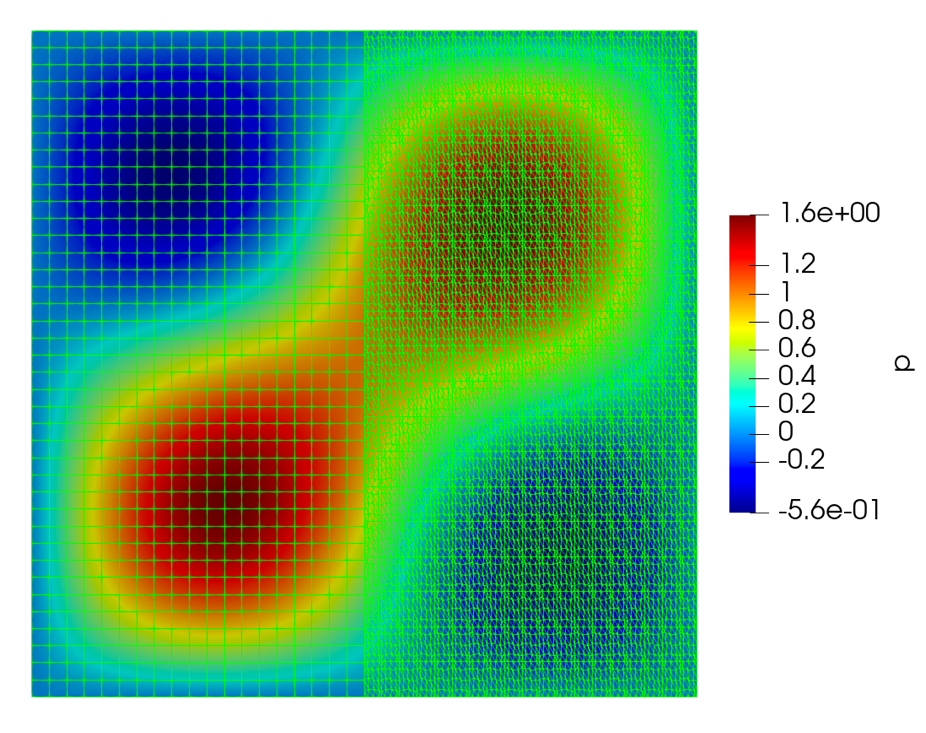
\includegraphics[width=0.8\linewidth,trim=4 4 4 4,clip]{figures/split_domain_wave.png}
\caption{Pressure initial condition for test problem, also showing split-domain
	 discretization.}
\label{fig:split_domain}
\end{figure}

Our success metrics for this test problem include
\begin{itemize}
\item{Demonstrating accurate recreation of the total energy of the system, as observed in the numerical simulation of the problem, via a total energy relation derived from the
spatial and interfacial schema.}
\item{Demonstrating that this energy does not increase (condition for semi-discrete stability).}
\item{Demonstrating the prescribed order of accuracy using L2 norms.}
\end{itemize}

Upon fulfillment of these goals, extension to three dimensions will be considered.

%===========================================================================
\subsection{Results}

%===========================================================================
\subsection{Outlook}

\subsubsection{Current Status}

\subsubsection{Risk Mitigation}

Should our goal of a new and unisolvent stable interface method not come to
fruition, a "fallback" goal of sorts is identified in that Kozdon and Wilcox's
method has yet to be extended to three dimensions. This would present more of a
technical challenge than an intellectual one, but a study of how the method
responds to certain geometric scenarios untestable in two dimensions (namely
three-dimensional corners) has potential to yield further information about
how the optimized operators perform numerically, as well as shed light on
optimization targets to yield better results in higher dimensions.

Furthermore, an additional unexplored topic that could prove to be a worthwhile
"fallback" goal - and one that potentially ties the two topics of this proposal
together - would be exploring the implications of the use of Kozdon and Wilcox's
projection operators on the timestep limitations of a given physical problem, and
(if a timestep disparity between the interior of a given subdomain and its interface
with another subdomain is identified) exposing this challenge to multi-rate Adams
integration.



%===========================================================================
